\documentclass[11pt, oneside]{article}   	% use "amsart" instead of "article" for AMSLaTeX format
\usepackage{geometry}                		% See geometry.pdf to learn the layout options. There are lots.
\geometry{letterpaper}                   		% ... or a4paper or a5paper or ... 
%\geometry{landscape}                		% Activate for for rotated page geometry
%\usepackage[parfill]{parskip}    		% Activate to begin paragraphs with an empty line rather than an indent
\usepackage{graphicx}				% Use pdf, png, jpg, or eps� with pdflatex; use eps in DVI mode
								% TeX will automatically convert eps --> pdf in pdflatex		
\usepackage{amssymb}
\usepackage{amsmath}
\usepackage{parskip}
\usepackage{color}

\title{Logarithmic differentiation}
%\author{The Author}
%\section{}
% \subsection*{R code}
\date{}							% Activate to display a given date or no date

\graphicspath{{/Users/telliott_admin/Dropbox/Tex/png/}}

% \begin{center} 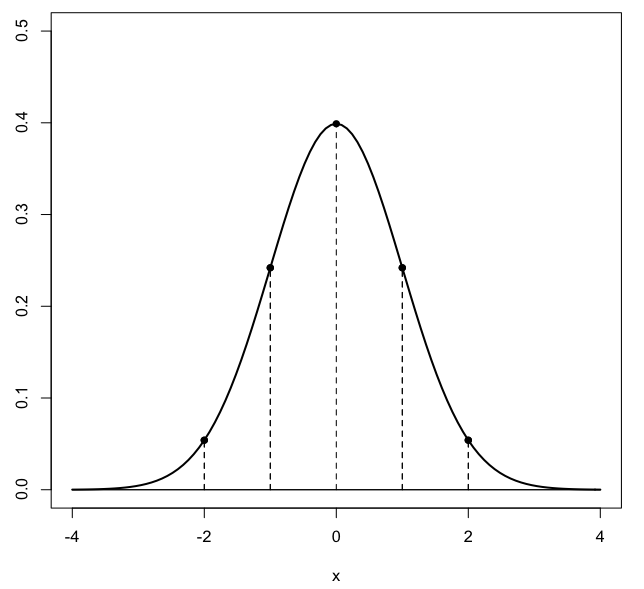
\includegraphics [scale=0.4] {gauss3.png} \end{center}
% \begin{bmatrix} a  &  b \\ c  &  d \end{bmatrix}
% \bigg |_

\begin{document}
\maketitle
\large
%\noindent

Here is the first problem Paul uses for this topic.  Differentiate

\[ y = \frac{x^5}{(1-10x)\sqrt{x^2+2}} \]

We could use the product, quotient and chain rules for this (and we can be sure it will be messy in the end).  An alternative is to use the properties of the logarithm to break the right-hand side into a polynomial.  Take the logarithm of both sides

\[ \ln y = \ln (\frac{x^5}{(1-10x)\sqrt{x^2+2}} ) \]
\[ \ln y = \ln(x^5) - \ln(1-10x) - \ln(\sqrt{x^2+2}) \]

Now, when we differentiate, it is really implicit differentiation.  Imagine that both $y$ and $x$ are functions of $t$ (e.g. $x=t$).  Then the one term from the left and three from the right are

\[ \frac{d}{dt} \ln y = \frac{1}{y} \frac{dy}{dt} \]
\[ \frac{d}{dt} \ln (x^5) = \frac{1}{x^5} 5x^4 \frac{dx}{dt}  = \frac{5}{x} \frac{dx}{dt}\]
\[ \frac{d}{dt} \ln (1-10x) = \frac{1}{(1-10x)} (-10) \frac{dx}{dt} = - \frac{10}{(1-10x)} \frac{dx}{dt}  \]
\[ \frac{d}{dt} \ln (\sqrt{x^2+2} = \frac{1}{\sqrt{x^2+2}} \frac{1}{2\sqrt{x^2+2}} 2x \frac{dx}{dt} = \frac{x}{x^2 + 2}  \frac{dx}{dt}  \]

Every term has $dt$ in the denominator, so that just cancels.  Bring the $dx$ from every term on the right to the left-hand side.  On the left we get
\[ \frac{1}{y} \frac{dy}{dx} = \frac{y'}{y}  \]
for the rest we have
\[ \frac{y'}{y} =   \frac{5}{x} + \frac{10}{(1-10x)} - \frac{x}{x^2 + 2} \]

To finish the problem, we need to multiply through by $y$

\[ y' = (\frac{x^5}{(1-10x)\sqrt{x^2+2}}) ( \frac{5}{x} + \frac{10}{(1-10x)} - \frac{x}{x^2 + 2}) \]

which I won't try to simplify.

Besides these (painful and rather silly) algebraic manipulations, the main thing about logarithmic differentiation is that it allows us to solve a problem we couldn't do until now.  Differentiate

\[ y = x^x = ? \]

Take the logarithm of both sides

\[ \ln y = \ln (x^x) = x \ \ln x \]

Now, we can differentiate

\[ \frac{y'}{y} = x (\frac{1}{x}) + \ln x (1) = 1 + \ln x \]
So 

\[ y' = x^x (1 + \ln x) \]



\end{document}  